\section{Syntax Tree Validation} % (fold)
\label{sec:syntax_tree_validation}
	As we only support a fairly limited set of C\#’s built-in constructs and types, it is important to make sure that users only make use of those that we are able to map to Script\#. Should users utilise one of the constructs or types that we are not able to map, this should be pointed out with an understandable error message. It should not be left to the users to debug or understand a Roslyn or Script\# exception. Furthermore, it is important to make sure that users use their own code correctly. The remainder of this section will describe how a Validator class is used to achieve this.

	As mentioned above, it is necessary to make sure that users only utilise C\# constructs (method declarations, various statements and expressions, etc.) that we can correctly map to Script\#. At the moment, this is handled by the Builder classes, and will be explained in a later section. However, optimally this should be the responsibility of the Validator class. How this can be achieved is described in future work. It should also be confirmed that users utilise types and their members correctly. This is handled by the validator class. It should be noted that currently only methods are supported as members.

	To explain correct usage of types and members, it is beneficial to divide them into two categories; the ones that are built into the .NET platform and the ones users define themselves. Understanding “correct usage of .NET built-in types and members” is straightforward; it means that users are only allowed to use the types and members that can be mapped correctly to Script\#. How this is achieved is described later in this section. However, “correct usage of the types defined by the users themselves” requires some explanation. For this, the MixedSide Principle is introduced.



	\subsection{Validating} % (fold)
	\label{sub:validating}

		There are essentially three situations in which it is necessary to verify correct usage of types and members. The first is object creation. When an instance of a type is created, it is necessary to check the type in question can be mapped. The second situation is when members on type instances are accessed. It is then necessary to check first if the type can be mapped, then if the type has a member corresponding to the one being accessed. The third is invocation of methods. It is then necessary to check if the invocation is done correctly, using the correct arguments and return type.

		The Validator class extends Roslyns SyntaxWalker class and it is thus able to traverse syntax nodes. The Validator takes a CompilationUnit which holds the code to be validated, a string containing an attribute name that decides what methods to validate, and a structure of types and members that the validated methods are allowed to use. It works by looking for classes in the CompilationUnit that contains methods annotated with the given attribute name and validates the body of these methods against the provided structure of members.

		The nature of the Validator requires the Syntax Tree to be validated twice. Once validating all the MixedSide methods against a structure containing all MixedSide types and their members, and once validating all the ClientSide methods against a structure containing all ClientSide types and members, MixedSide types and members and ScriptSharp DOM types and members. This is easily done by creating two instances of the Validator and validating them both, as shown in figure X. In the example, the ScriptSharp DOM types are already contained in the clientSideMembers. 

		\begin{figure}[H]
			\begin{center}
				\centerline{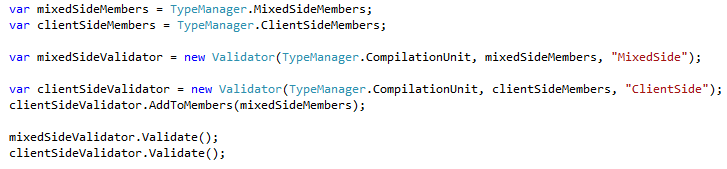
\includegraphics[width=14cm]{resources/images/validatorInitiation.png}}
			\end{center}
			\caption{Initiating the Syntax Tree Validation process}
			\label{validatorInitiation}
		\end{figure}

		The Validation process is best explained by looking at an example. Consider the situation showed in Figure \ref{fig:mixedSideValidationExample}. 

		\begin{figure}[H]
			\begin{center}
				\centerline{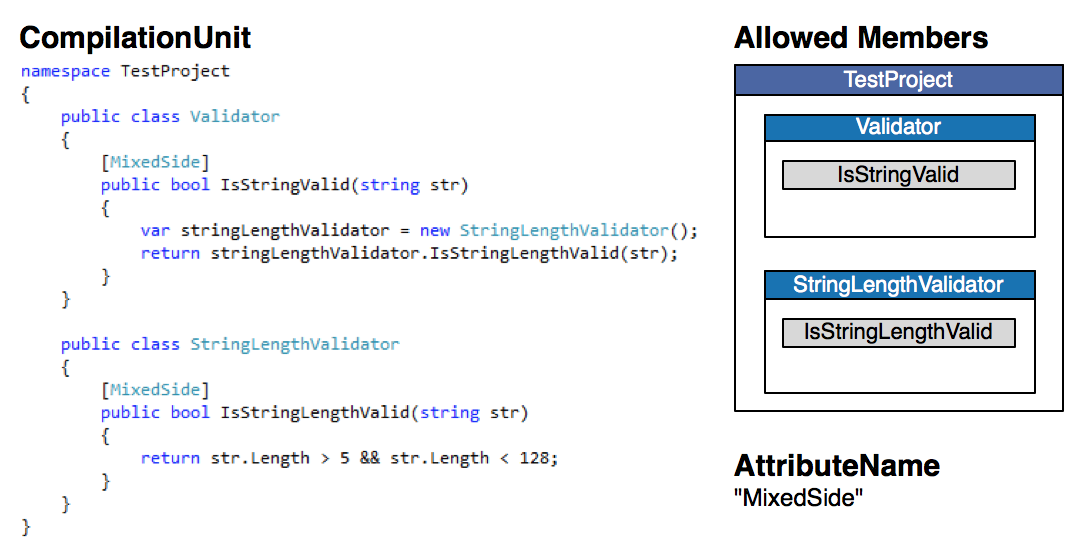
\includegraphics[width=14cm]{resources/images/MixedSideValidationExample.png}}
			\end{center}
			\caption{Initiating the Syntax Tree Validation process}
			\label{fig:mixedSideValidationExample}
		\end{figure}		
		
		The Validator traverses the CompilationUnit depth-first and discovers the Validator class. It then finds all of the Validator class's methods and loops through these to see if they have the MixedSide attribute. When a method annotated with the MixedSide attribute is found, the validator visits it straight away, as shown in Figure \ref{fig:ValidatorVisitClassDeclaration}. 

		\begin{figure}[H]
			\begin{center}
				\centerline{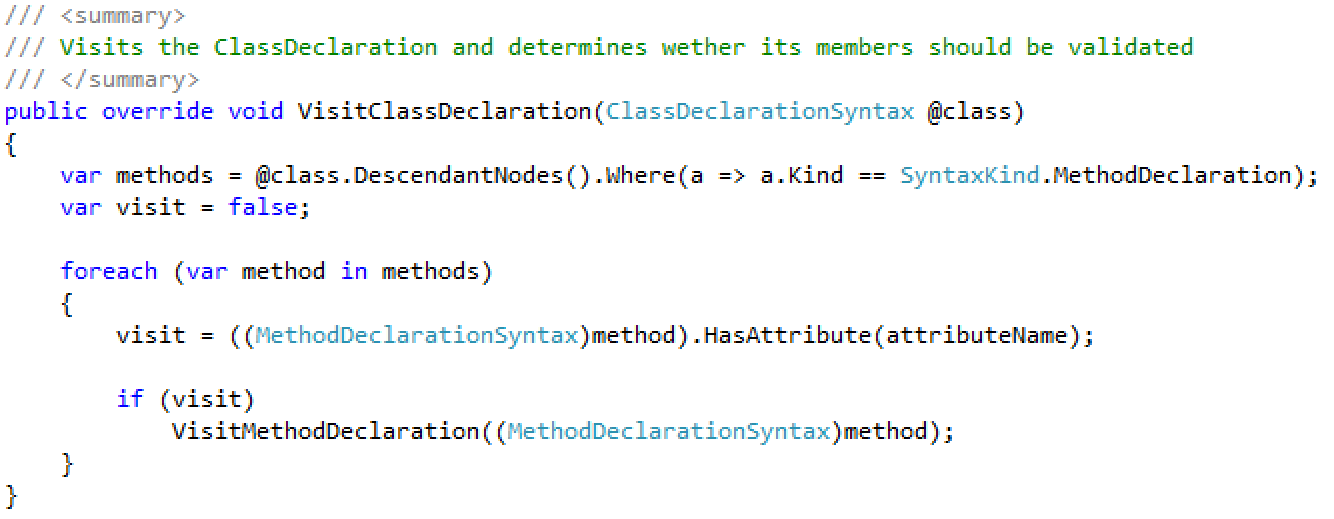
\includegraphics[width=14cm]{resources/images/ValidatorVisitClassDeclaration.png}}
			\end{center}
			\caption{Visiting a ClassDeclaration and deciding whether its methods should be validated or not}
			\label{fig:ValidatorVisitClassDeclaration}
		\end{figure}

		The first method visited is the \texttt{IsStringValid()} method. The first statement of the method contains an object creation expression and the Validator now needs to check if the object creation is legal. It is legal either if the created object is a supported core type, or if the object is a user defined MixedSide type (residing within the members structure). As the type exists in the allowed members structure (shown in figure \ref{fig:mixedSideValidationExample}) the object creation is legal and the traversal continues. If it had not existed in the allowed member structure (this could happen if it had been ClientSide), and had not been a supported core type, the MixedSide Principle would have been violated, and an exception of type \texttt{MixedSidePrincipleViolatedException} had been thrown.

		The validation of a member access is done in a very similar way, only checking if the member exists in the allowed-members structure or in the core mapping as well.

		TODO: Write about how invociations are validated: Only core types need to be validated (with arguments and return types), as user types will automatically be validated by the compiler.


% \begin{lstlisting}[language=CSharp,classoffset=1,morekeywords={TextBox,Panel,CheckBox, Button}]
% TextBox NameBox = new TextBox() { ID = "name", Text = "Name" };
% Panel CheckBoxGroup = new Panel();
% CheckBox SnailMailCheck = new CheckBox() { ID = "dmSnailmail", Text = "Snail Mail" };
% CheckBox EmailCheck = new CheckBox() { ID = "dmEmail", Text = "E-Mail" };
% TextBox AddressBox = new TextBox() { ID = "address", Text = "Address" };
% TextBox ZipcodeBox = new TextBox() { ID = "zipcode", Text = "Zip Code" };
% TextBox EmailBox = new TextBox() { ID = "email", Text = "E-mail" };
% TextBox PhoneBox = new TextBox() { ID = "phone", Text = "Phone" };
% Button SubmitButton = new Button() { Text = "Register" };
% \end{lstlisting}






	
	% subsection validating (end)
% section syntax_tree_validation (end)